\section{Introduction}

\begin{frame}[fragile]{Introduction}
	
	The aim of the project was to mimic the people's behavior in a big city. It tackles the following problematics :
	\begin{itemize}
		\item What do people do in their everyday life and at what time ?
		\item In what kind of environment do they live and how do they interact with the infrastructures ?
	\end{itemize}
	Tools we used :
	\begin{figure}
		\centering
		\begin{subfigure}{.24\textwidth}
			\centering
			
\includegraphics[width=.5\linewidth]{images/python.png}
		\end{subfigure}%
		\begin{subfigure}{.24\textwidth}
			\centering
			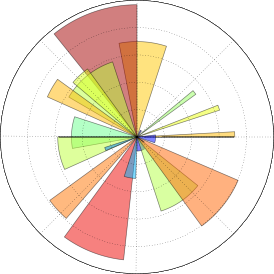
\includegraphics[width=.5\linewidth]{images/matplotlib.png}
		\end{subfigure}%
		\begin{subfigure}{.24\textwidth}
			\centering
			
\includegraphics[width=.5\linewidth]{images/sympy.png}
		\end{subfigure}%
		\begin{subfigure}{.24\textwidth}
			\centering
			
\includegraphics[width=.5\linewidth]{images/sklearn.png}
		\end{subfigure}
	\end{figure}
\end{frame}

\section{Transportation network}
\subsection{Topology}
\begin{frame}{Topology -- main steps}
	We tried to model a subway network similar to the Parisian one.
	\begin{block}{Steps}
		\begin{enumerate}
			\item \textbf{Terminals} : subway lines modeled as segments.
			\item \textbf{Intersections} : intersections between lines are glued together if they are close.
			\item \textbf{Stations} : points at regular intervals (with a little noise).
			\item \textbf{Hubs} : stations crossed by many lines
			\item \textbf{Fast lines} : a few lines that connect close hubs together.
		\end{enumerate}
	\end{block}
\end{frame}

\begin{frame}{Topology -- illustrations}
	\begin{figure}
		\centering
		\captionsetup{justification=centering}
			
		\begin{subfigure}[t]{.3\textwidth}
			\centering
			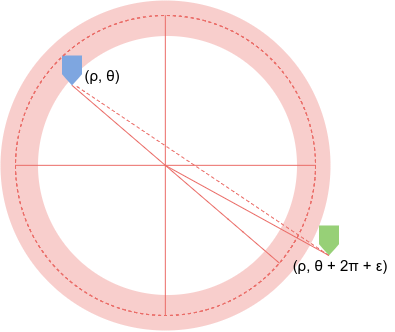
\includegraphics[width=0.8\linewidth]{images/create_line.png}
			\caption{Terminals : originate in the suburbs, go through the center}
		\end{subfigure}\qquad%
		\begin{subfigure}[t]{.3\textwidth}
			\centering
			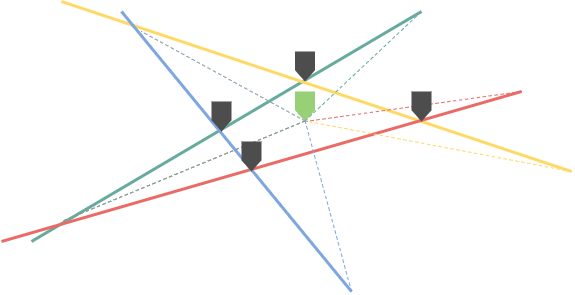
\includegraphics[width=\linewidth]{images/glue_intersections.png}
			\caption{Intersections : move close intersections to their centroid}
		\end{subfigure}\qquad%
		\begin{subfigure}[t]{.3\textwidth}
			\centering
			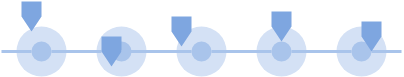
\includegraphics[width=\linewidth]{images/station_creation.png}
			\caption{Stations : sample the line and add noise}
		\end{subfigure}
	\end{figure}
\end{frame}

\begin{frame}{Topology -- results}
	\begin{figure}
		\centering
		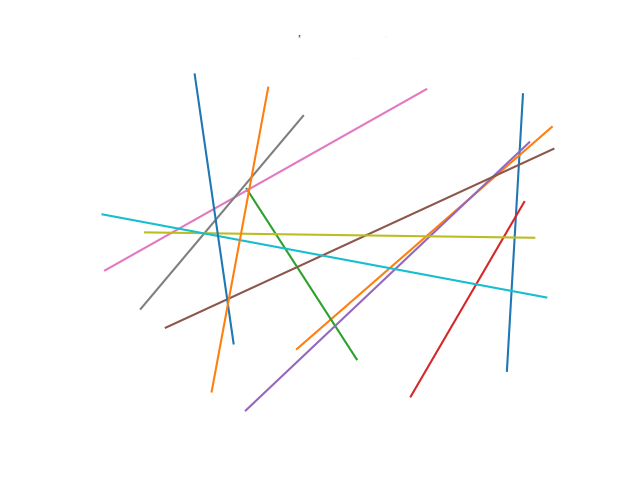
\includegraphics[width=0.7\linewidth]{images/net_1.png}
		\caption{Terminals generation -- subway lines are simple segments}
	\end{figure}
\end{frame}
\begin{frame}{Topology -- results}
	\begin{figure}
		\centering
		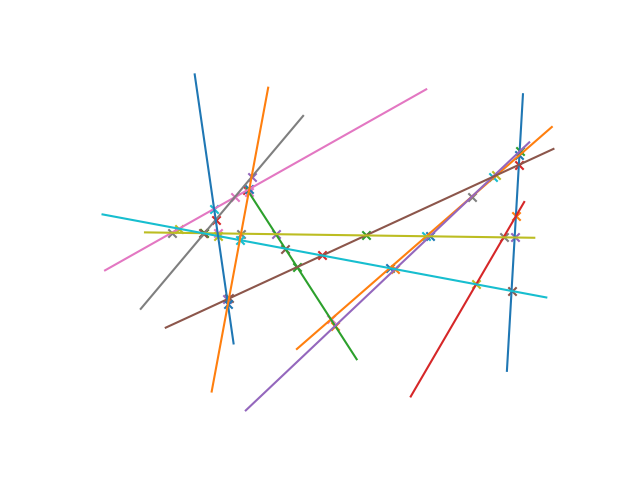
\includegraphics[width=0.7\linewidth]{images/net_2.png}
		\caption{Intersection resolution -- find where the lines cross using SymPy}
	\end{figure}
\end{frame}
\begin{frame}{Topology -- results}
	\begin{figure}
		\centering
		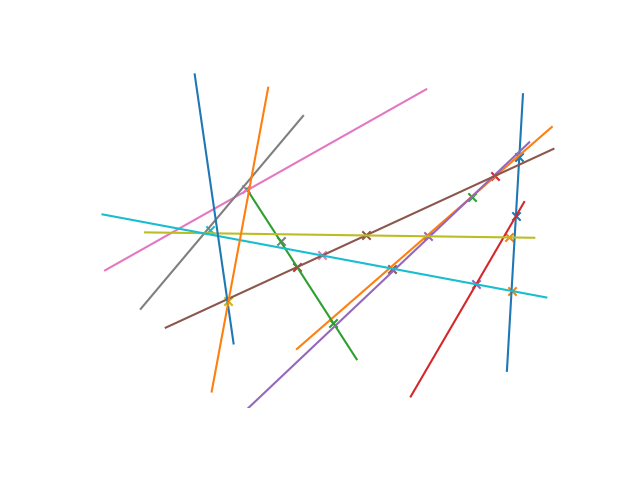
\includegraphics[width=0.7\linewidth]{images/net_3.png}
		\caption{Intersection gluing -- merge close intersections using a clustering algorithm (DBSCAN)}
	\end{figure}
\end{frame}
\begin{frame}{Topology -- results}
	\begin{figure}
		\centering
		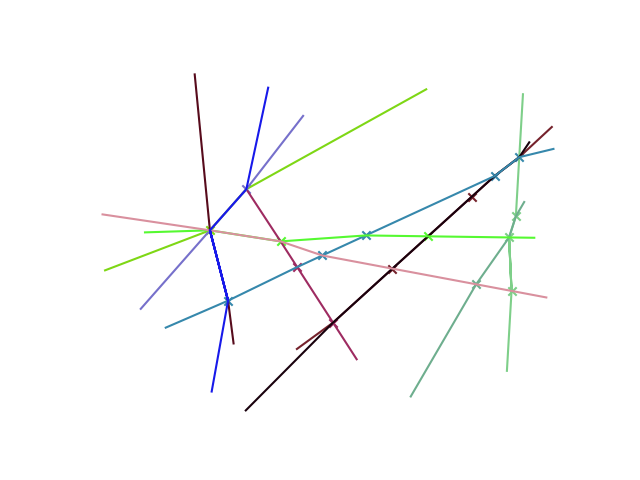
\includegraphics[width=0.7\linewidth]{images/net_4.png}
		\caption{Line bending -- bend te lines such that they cross glued intersections}
	\end{figure}
\end{frame}
\begin{frame}{Topology -- results}
	\begin{figure}
		\centering
		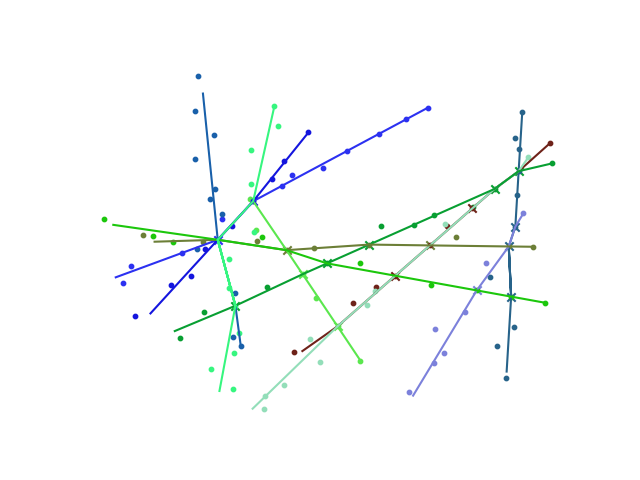
\includegraphics[width=0.7\linewidth]{images/net_5.png}
		\caption{Stations -- put stations at regular intervals plus a little noise}
	\end{figure}
\end{frame}
\begin{frame}{Topology -- results}
	\begin{figure}
		\centering
		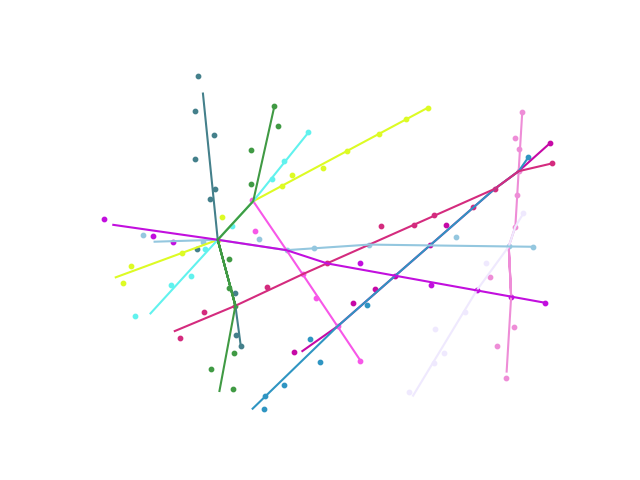
\includegraphics[width=0.7\linewidth]{images/net_6.png}
		\caption{Stations gluing -- merge close intersections with DBSCAN again}
	\end{figure}
\end{frame}
\begin{frame}{Topology -- results}
	\begin{figure}
		\centering
		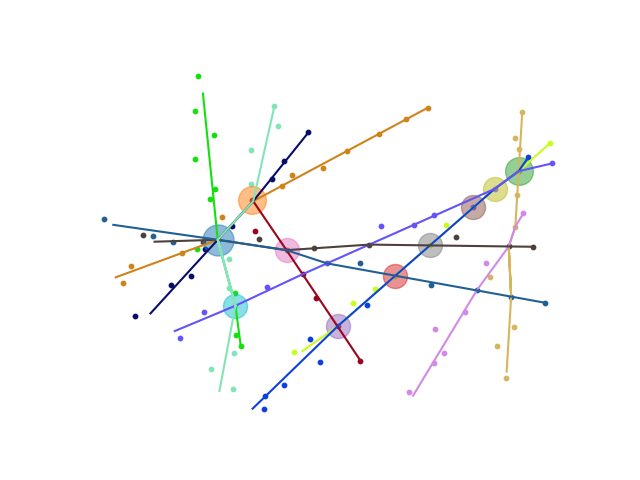
\includegraphics[width=0.7\linewidth]{images/net_7.png}
		\caption{Hubs -- find stations with many lines crossing them and generate fast lines}
	\end{figure}
\end{frame}


\subsection{Toponymy}
\begin{frame}{Toponymy -- main steps}
	Generate a ``realistic'' name for each station, like ``Place Edith Piaf'', ``Rue de la Chine'' or ``Saint Marcel''
	\begin{block}{Steps}
		\begin{enumerate}
			\item \textbf{Data collection} : collect names from databases (country names, first names) or manually (famous people).
			\item \textbf{Combine elements together} : use link words (``Place de la/le'', ``Saint(e)'', ``-''...) appropriately.
			\item \textbf{Do some tricks} : avoid things like ``Place d'Arc'' or ``Avenue de Maupassant''... 
		\end{enumerate}
	\end{block}
	\textbf{``Best-of''} : ``Avenue Johnny Hallyday'', ``Gare Nabilla'', ``Rue du Swaziland''...
\end{frame}

\begin{frame}
		\begin{figure}
			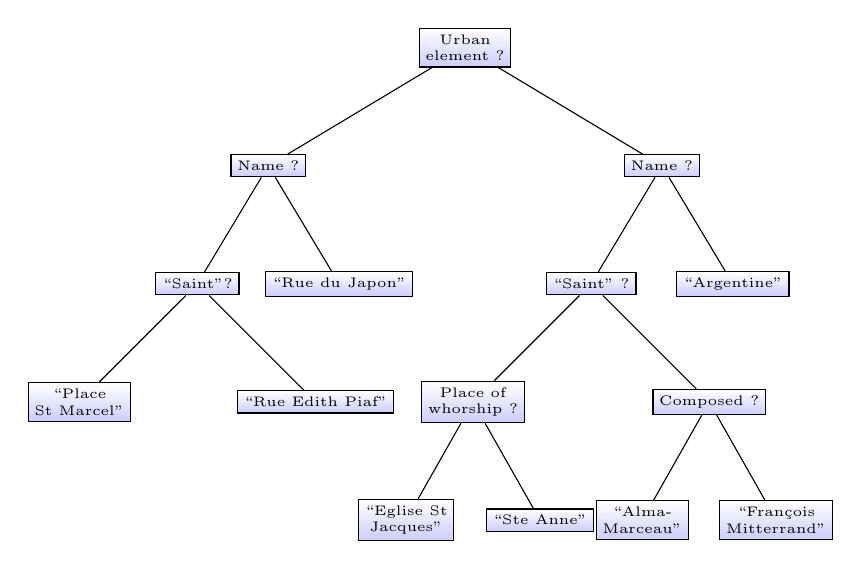
\begin{tikzpicture}[
		level 1/.style={sibling distance=50mm},
		level 2/.style={sibling distance=18mm},
		level 3/.style={sibling distance=30mm},
		level 4/.style={sibling distance=17mm},
		level 5/.style={sibling distance=10mm},
		every node/.style = {shape=rectangle,
			draw, align=center,
			top color=white, bottom color=blue!20}]
		\tiny
		\node {Urban \\ element ?}
		child { node {Name ?}
			child { node {``Saint''?}
				child { node {``Place \\ St Marcel''}}
				child { node {``Rue Edith Piaf''}}}
			child { node {``Rue du Japon''} } }
		child { node {Name ?} 
			child { node {``Saint'' ?}
			child { node {Place of\\whorship ?}
				child { node {``Eglise St\\ Jacques''} }
				child { node {``Ste Anne''} }}
			child { node {Composed ?}
				child { node {``Alma-\\Marceau''}}
				child { node {``François\\ Mitterrand''}}
			} 
			}
		child { node {``Argentine''}}}
;
		\end{tikzpicture}
		\caption{Simplified binary tree for name generation}
		\end{figure}
\end{frame}

\subsection{Schedule}
\begin{frame}{Schedule -- main steps}
	Generate a schedule for each station and deduce point to point travel times.
	\begin{block}{Steps}
		\begin{enumerate}
		\item Compute travel times between stations, depending on the line speed and the distances between stations.
		\item Generate departure times from the terminals with a frequency that varies during the day.
		\item Propagate the departure times along the line using the values computed at first step.
		\item Use the schedule to compute a shortest path that is sensitive to de day/hour of departure (\textbf{not implemented})
		\end{enumerate}
	\end{block} 
\end{frame}
\begin{frame}{Schedule --  illustration}
	\begin{figure}
		\centering
		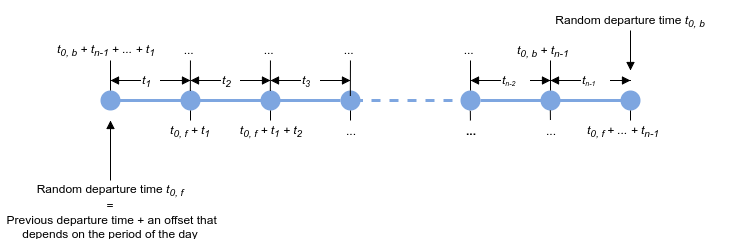
\includegraphics[width=\linewidth]{images/schedule.png}
		\caption{Computation of a line of the schedule for one subway line}
	\end{figure}
\end{frame}